\section{Burndown Charts}
\subsection*{Sprint Burndown}

En el sprint burndown mostramos como fuimos resolviendo las tareas en nuestro sprint basandonos en los story points como medida.
Aca estamos considerando como terminada una tarea cuando ya teniamos la forma de resolver, aunque no necesariamente este implementado.
Decidimos mostrarlo asi, ya que muestra mejor el proceso del desarrollo del trabajo pr\'actico.

La linea rojo representa un proceso de desarrollo \emph{ideal} que no representa necesariamente un proceso de desarrollo posible, pero
sirve como guia para poder ver el desvio del desarrollo actual.
En linea azul vemos el desarrollo del equipo durante el sprint. Cabe destacar, tal como mencionamos en la secci\'on de sprint backlog, que
nuestro sprint abarca el tiempo entre la presentaci\'on del tp y la fecha de entrega.

Se puede observar del gr\'afico que adquirimos m\'as velocidad al acercarse la fecha de entrega. Esto en parte se debe tambien a que no mostramos
tareas como la elaboraci\'on del sprint y product backlog. Tambi\'en vemos que durante la semana del parcial bajamos la velocidad
debido a que no pudimos dedicarnos al trabajo pr\'actico. Por \'ultimo hubo una tarea del sprint backlog que al final decidimos que
no era necesaria de implementar para mostrar la funcionalidad escencial.

\begin{figure}[H]
\begin{center}
 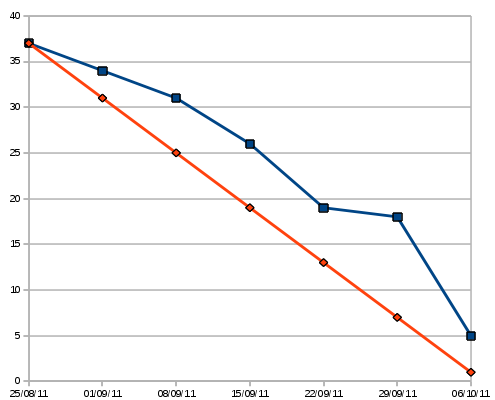
\includegraphics[scale=0.6]{burn3.png}
\end{center}
\end{figure}
\newpage
\subsection*{Product Burndown}

En el product backlog mostramos el avance de la implementaci\'on basandonos en el business value de cada story.
Nuevamente mostramos en rojo un proceso de desarrollo \emph{ideal} y en azul el proceso de desarrollo del equipo.
Las primeras semanas tuvimos mucha inactividad debido a que estuvimos m\'as tiempo pensando el dise\~no de objetos.
Adem\'as nos falto implementar el story del hasheo de contrase\~nas porque consideramos que no era necesario para mostrar el
funcionamiento para la demo.

\begin{figure}[H]
\begin{center}
 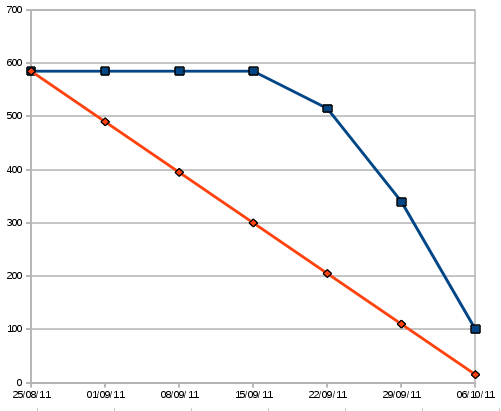
\includegraphics[scale=0.6]{burn1.png}
\end{center}
\end{figure}
